\documentclass{beamer}
\usepackage[utf8]{inputenc}
\usepackage[export]{adjustbox}
\usepackage{hyperref}
\hypersetup{
	colorlinks=true,
	urlcolor=adcorange,
	linkcolor=adcblue
}

\usetheme{Madrid}

\title{Let's make a todo list app with React Native!}
\subtitle{Components and styling!}
\author{Nathaniel Budijono}
\date{February 1, 2022}
\institute{UMN ADC}

\definecolor{adcblue}{RGB}{115,203,255}
\definecolor{adcorange}{RGB}{242,114,0}

\setbeamercolor{palette primary}{fg=white,bg=adcblue}
\setbeamercolor{palette secondary}{fg=adcorange,bg=white}
\setbeamercolor{structure}{fg=adcblue,bg=white}
\setbeamercolor{title in head/foot}{fg=adcblue,bg=white}
\setbeamercolor{date in head/foot}{fg=gray,bg=white}
\setbeamercolor{palette tertiary}{fg=white,bg=adcorange}

\begin{document}

\begin{frame}
    \titlepage
    \includegraphics[width=0.25\textwidth, right]{figs/ADC_Logo_Blue.png}
\end{frame}

\begin{frame}{Announcements}
	Developer mixer this Thursday, Feb 3 from 6-7pm at Tate Hall 120! Meet potential collaborators!

	\bigskip

	If you're here in person, feel free to get food!	
\end{frame}

\begin{frame}{Officer openings!}
	\begin{itemize}
		\item Workshop instructors
	\end{itemize}

	\bigskip

	DM us on the discord!

	\bigskip

	\href{https://z.umn.edu/ADCdiscord}{https://z.umn.edu/ADCdiscord}
\end{frame}

\begin{frame}{Guide}
	We will be following this guide: \href{https://github.com/ADC-UMN/todotorial}{https://github.com/ADC-UMN/todotorial}. Feel free to go ahead of the workshops at your own pace.
\end{frame}

\begin{frame}{What we're starting with}
	\centering
	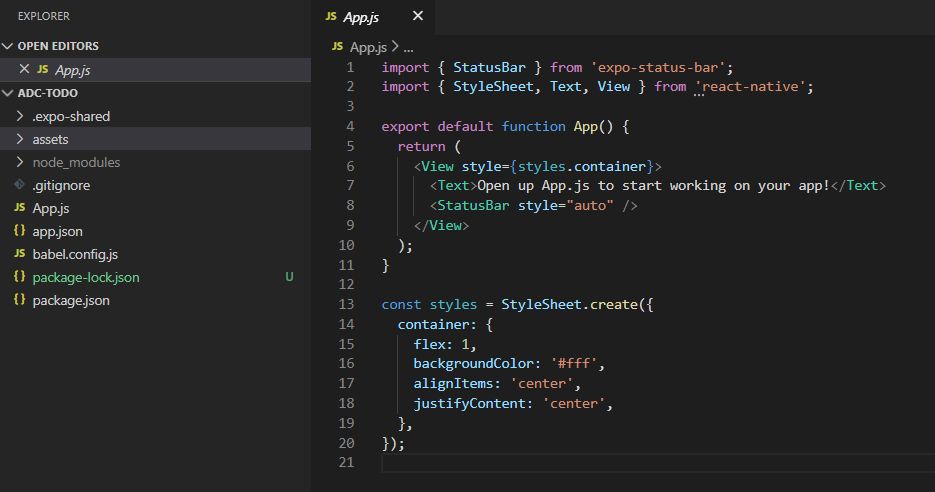
\includegraphics[width=0.9\textwidth]{figs/expo-blank.png}	
\end{frame}

\begin{frame}{Imports}
	\begin{itemize}
		\item \texttt{Text}
		\item \texttt{View}
		\item \texttt{FlatList}
		\item \texttt{Button}
		\item \texttt{TextInput}
		\item \texttt{StyleSheet}
		\item \texttt{AsyncStorage}
		\item \texttt{ActivityIndicator}
	\end{itemize}
\end{frame}

\begin{frame}{Class component boilerplate}
	\texttt{export default class App extends React.Component \{ ... \}}\pause

	\bigskip

	Now let's implement \texttt{render()}!
\end{frame}

\begin{frame}{Constructor and props}
	Let's look at the documentation to plan out our constructor and how we use our components: \href{https://reactnative.dev/docs/components-and-apis}{https://reactnative.dev/docs/components-and-apis}

	\bigskip\pause

	\begin{itemize}
		\item \texttt{FlatList} \pause
		\item \texttt{TextInput} for next workshop!
	\end{itemize}
\end{frame}

\begin{frame}{Stylesheets}
	Let's explore styling in React Native! \href{https://reactnative.dev/docs/style}{https://reactnative.dev/docs/style} \pause

	\bigskip

	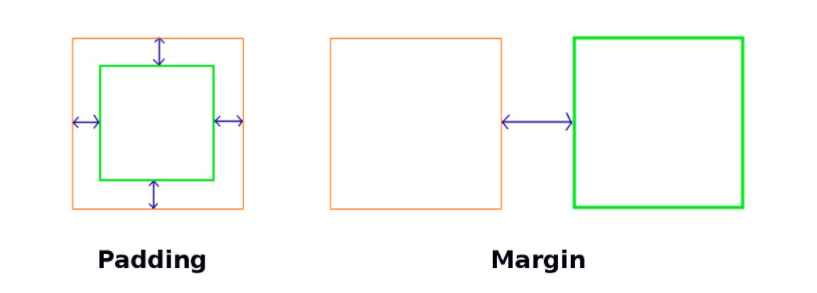
\includegraphics[width=0.9\textwidth]{figs/padding-margin.png}

	\pause\bigskip

	Flex is also quite confusing... \href{https://reactnative.dev/docs/flexbox}{https://reactnative.dev/docs/flexbox}
\end{frame}

\end{document}